%%Author of assignment template: Jeff Patterson

\documentclass[10pt,letterpaper, cm]{hmcpset}
\usepackage[utf8]{inputenc}
\usepackage{biblatex}
\usepackage{amsmath}
\usepackage{multicol}
\usepackage{amsthm}
\usepackage{cancel}
\usepackage{enumerate}
\usepackage{graphicx}
\usepackage{tikz}
\usepackage{fullpage}
\usetikzlibrary{arrows,	petri, topaths}
				
\usepackage{tkz-berge}
\usepackage{tkz-graph}
\assignment{Graph Theory Knowledge}
\name{Jonathon Sonesen }
\setlength{\columnsep}{0.5cm}
\setlength{\columnseprule}{00pt}
\date{May 2015}
\extra{Collaborators: Jeff Patterson, Steven Whetherbee, Kyle Kneitenger}
\begin{document}

\begin{problem}[1]
  Let $G$ be a simple graph with $n$ nodes. Let $k$ be the number of edges of $G$
  \[
    k \leq \frac{n(N-1)}{2}
  \]
\end{problem}  

\begin{problem}[2]
  Let $G$ be the graph:
  \begin{center}  
  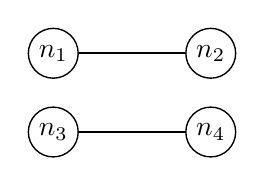
\begin{tikzpicture}[scale=1,transform shape]

      \GraphInit[vstyle=Dijkstra]
      \SetVertexMath
      \Vertex[x=0,y=0]{n_1}
      \Vertex[x=2,y=0]{n_2}
      \Vertex[x=0,y=-1]{n_3}
      \Vertex[x=2,y=-1]{n_4}
      \Edge[](n_1)(n_2)
      \Edge[](n_3)(n_4)
    \end{tikzpicture}
\end{center}
  What is the complement of $G$?
\end{problem}


\begin{problem}[3]
List a simple graph that has 4 nodes of different degree, or prove that no such graph exists.
\end{problem}

\begin{problem}[4]
  What is the maximum nuumber of edges possible in a disconnected graph of $n$ nodes and no loops
  or parellel esges? Explain your answer(no proof needed)
\end{problem}


\begin{problem}[5]
  Let $G$ be the graph:
  \begin{center}
    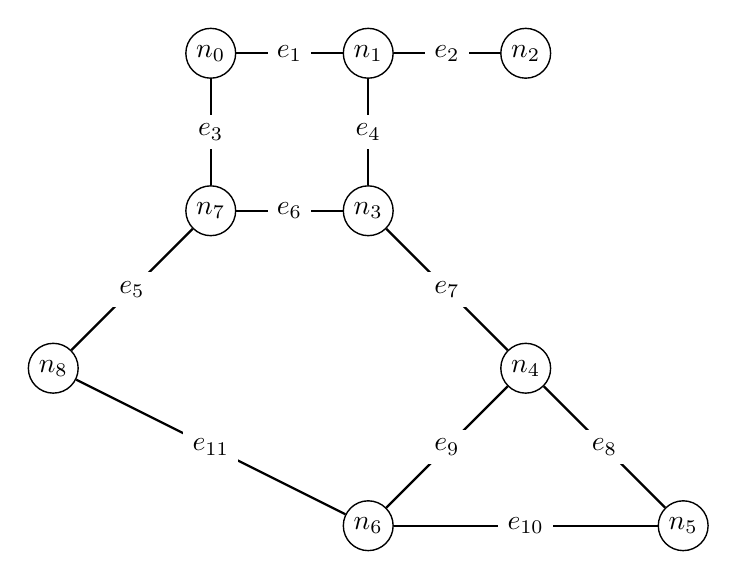
\begin{tikzpicture}[scale=1, transform shape]
      \GraphInit[vstyle=Dijkstra]
      \SetVertexMath

      \Vertex[x=0, y=0]{n_0}
      \Vertex[x=2, y=0]{n_1}
      \Vertex[x=4, y=0]{n_2}
      \Vertex[x=2, y=-2]{n_3}
      \Vertex[x=4, y=-4]{n_4}
      \Vertex[x=6, y=-6]{n_5}
      \Vertex[x=2, y=-6]{n_6}
      \Vertex[x=0,  y=-2]{n_7}
      \Vertex[x=-2, y=-4]{n_8}
      \Edge[label=$e_1$](n_0)(n_1)
      \Edge[label=$e_2$](n_1)(n_2)
      \Edge[label=$e_3$](n_0)(n_7)
      \Edge[label=$e_4$](n_1)(n_3)
      \Edge[label=$e_5$](n_7)(n_8)
      \Edge[label=$e_6$](n_7)(n_3)
      \Edge[label=$e_7$](n_3)(n_4)
      \Edge[label=$e_8$](n_4)(n_5)
      \Edge[label=$e_9$](n_4)(n_6)
      \Edge[label=$e_{10}$](n_6)(n_5)
      \Edge[label=$e_{11}$](n_6)(n_8)
      
    \end{tikzpicture}
  \end{center}
  \begin{enumerate}
    \item List the adjacency matrix for this graph
    \item List the incidence matrix for this graph
  \end{enumerate}
\end{problem}



\end{document}
